\section{Zielsetzung}
In diesem Versuch wird der Franck-Hertz-Versuch untersucht.
Mit ihr können diskrete Energiewerte eines Atoms bestimmt werden. Des Weiteren wird
die Energieverteilung von Elektronen sowie die Ionisationsenergie von Quecksilber (Hg) untersucht und bestimmt.
\section{Theorie}
Unter Elektronenstoßexperiment gehört der der Frank-Hertz-Versuch dazu. Sie dient zur Strukturaufklärung
der Elektronenhülle.
In einen abgeschlossenen Raum lässt sich monoenergetische Elektronen mit darin enthaltenden Hg-Dampf wechselwirken.
Es treten elastische und unelastische Stöße zwischen den beiden Materien statt.
Mit Hilfe der Energieerhaltung und Impulserhaltung aus der Mechanik kann die Energiedifferenz $\Delta E$,
die das Hg-Atom aufgenommen hat, berechnen.
Im Fall des unelastischen und elastischen Stoßes gilt die Formel:
\begin{equation}
  \frac{m_0 \cdot v_{vor}^2}{2} - \frac{m_0 \cdot v_{nach}^2}{2} = E_1 - E_0 = \Delta E
\label{eq:1}
\end{equation}
Dabei ist $E_1$ der erste angeregte Zustand und $E_0$ der Grundzustand.
\subsection{Aufbau des Franck-Hertz-Versuches}
In Abbildung (\ref{abb:1}) ist eine schematische Darstellung des Versuches zu sehen.
\begin{figure}[H]
\centering
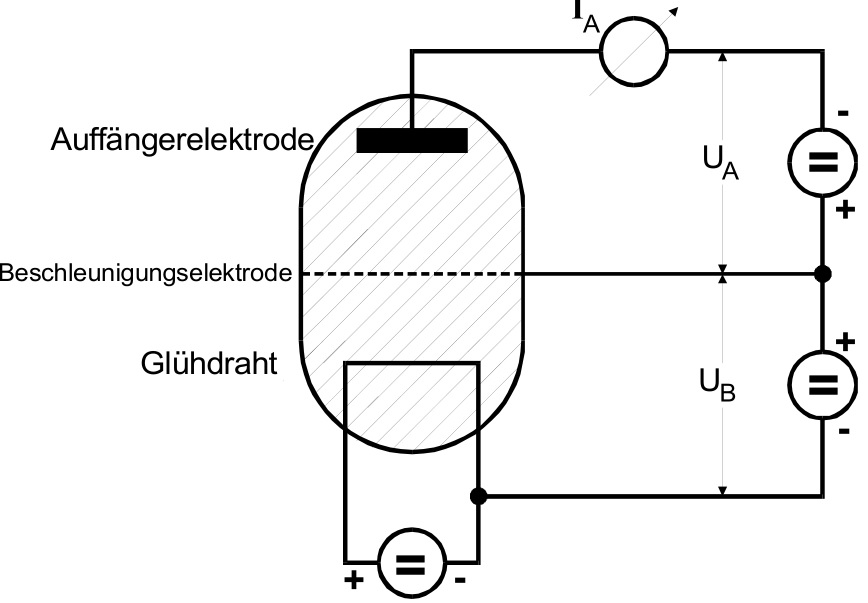
\includegraphics[width =7 cm, height = 5.5cm]{content/Aufbau.jpg}
\caption{Aufbau des Franck-Hertz-Versuches \cite{1}.}
\label{abb:1}
\end{figure}
Im evakuierten Gefäß befindet sich ein winziger Tropfen Quecksilber, der spontan verdampft. Es herrscht im Inneren ein
Gleichgewicht zwischen Druck und Temperatur. Der Druck, auch genannt als Sättigungsdruck $p_{sätt}$, ist nun
von der Umgebungstemperatur $T$ abhängig.
Im Glühdraht wird ein Gleichstrom angelegt und mit Hilfe des glühelektrischen Effektes treten dabei eine große Anzahl von
Elektronen aus. Die Beschleunigungsspannung ist von außen mit einer positiven Spannung $U_a$ angelegt.
Sobald Elektronen die Beschleunigungsstrecke durchlaufen, erhalten sie kinetische Energie.
Diese kinetische Energie lässt sich mit der Formel (\ref{eq:2} beschreiben:
\begin{equation}
  \frac{m_0 \cdot v_{vor}^2} {2} = e_0 \cdot U_b
  \label{eq:2}
\end{equation}
Dabei ist $e_0$ die Elementarladung. Zu beachten ist, dass die Gleichung (\ref{eq:2}) nur dann gilt, wenn
die Anfangsgeschwindigkeit aller Elektronen $0$ ist.
Sobald Elektronen zur Auffängerelektrode kommen, fließt ein Strom $I_A$ die gemessen werden kann.
Da eine Gegenspannung $U_A$ anliegt, entsteht ein Bremsfeld für die Elektronen und dabei können nur Elektronen in Feldrichtung (Z-Richtung) ankommen.
Es muss daher die Ungleichung
\begin{equation*}
  \frac{m_0 \cdot v_{z}^2} {2} \geq e_0 \cdot U_A
\end{equation*}
erfüllen.\\
Im Gefäß kommt es zwischen den Elektronen und den Hg-Atomen zu verschiedenen Stößen.
Ist die Energie der Elektronen zu gering, treten nur elastische Stöße auf. Aufgrund des großen
Masseunterschiedes zwischen Atom und Elektron ist die Energieabgabe $\Delta E \approx \num{1.1 e-5} E$
sehr gering.
Durch Erhöhung der Spannung $U_b$ können die Elektronen das Hg-Atom im ersten Zustand anregen.
Dabei überträgt es eine Energiedifferenz von $E_1 - E_0$ und behält das Elektron eine Restenergie von  $E -(E_1 -E_0)$.
Im angeregten Zustand des Hg-Atoms geht es nach einer Relaxationszeit in den Grundzustand zurück und
emittiert dabei ein Lichtquant dessen Energie
\begin{equation}
  h \cdot \nu = E_1 -E_0
\label{eq:3}
\end{equation}
beträgt.
Hier ist $h$ das Planck‘sche Wirkungsquantum und $\nu$ die Frequenz der emittierten Strahlung.
Die Anregung des Hg-Atoms folgt dadurch, dass sich die Beschleunigungsspannung $U_b$ größer ist als die
fest eingestellt Gegenspannung $U_a$ ist und ein Strom $I_a$ fließt kann.
In Abbildung (\ref{abb:2})
\begin{figure}[H]
\centering
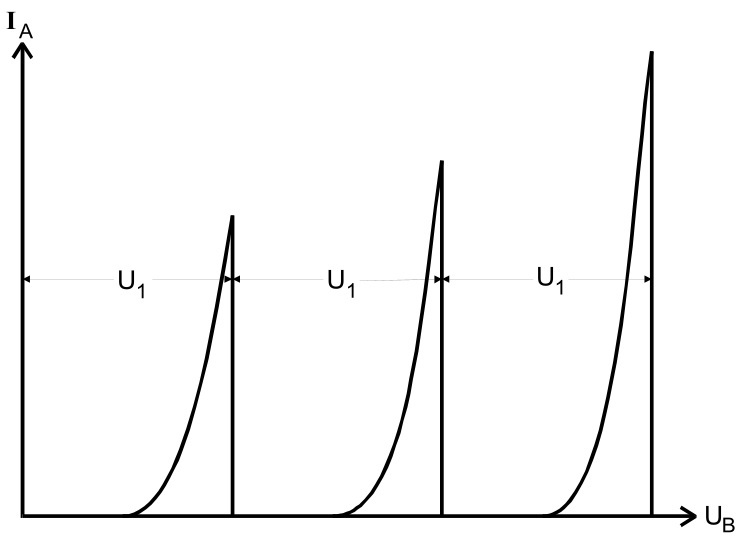
\includegraphics[width =7 cm, height = 5.5cm]{content/Verlauf.jpg}
\caption{Schematische Darstellung der Franck-Hertz-Kurve \cite{1}.}
\label{abb:2}
\end{figure}
ist ein idealisierter Zusammenhang zwischen dem Auffängerstrom $I_A$ und
der Beschleunigungsspannung $U_b$ abgebildet.
Der Verlauf der Kurve sagt aus, dass sobald die Elektronenenergie den Energiedifferenzwert $E_1 - E_0$ erreicht hat, treten
unelastische Stöße auf und die Elektronen verlieren ihre Energie und die Auffängerelektrode detektiert kein Strom $I_A$ mehr.
Durch Erhöhung der Beschleunigungsspannung $U_b$ bekommen die Elektronen erneut Energie dazu.
Sobald die Elektronen wieder die Energiedifferenz erreichen haben treten erneut unelastische Stöße auf und der Vorgang wiederholt sich.
Wie in der Abbildung (\ref{abb:2}) erfolgt dies in einem periodischen Intervall ab und
der Abstand $U_1$ bezeichnet das erste Anregungspotential:
\begin{equation}
  U_1 = \frac{1}{e_0} \cdot (E_1 - E_0)
  \label{eq:4}
\end{equation}
des Hg-Atoms.
\subsection{Störeinflüsse}
Die Kurve in Abbildung (\ref{abb:2}) weicht in folgenden Punkten ab, da einige Nebeneffekte berücksichtigt werden müssen.
Zum einen ist die Austrittsarbeit für die Elektronen eines Glühdrahts vom Material abhängig.
Es sollte daher ein Material ausgesucht werden, dessen Austrittsarbeit $\Phi_g$ kleiner ist als die
Austrittsarbeit der Beschleunigungselektrode $\Phi_b$.
Es ergibt sich nun für das effektive Beschleunigungspotential $U_\text{b,eff}$ den folgenden Ausdruck:
\begin{equation}
  U_{b,eff} = U_b - \frac{1}{e_0} \cdot (\Phi_b - \Phi_g)
  \label{eq:5}
\end{equation}
Der letzte Term wird auch als Kontaktpotential $K$ bezeichnet.
Das Kontaktpotenzial verschiebt lediglich die Franck-Hertz-Kurve nach vorne oder nach hinten.\\
Des Weiteren sind die Elektronen beim Durchlaufen nicht monoenergetisch.
Die Austrittselektronen besitzen eine Energieverteilung mit verschiedenen Anfangsgeschwindigkeiten.
Dies führt dazu, dass die unelastischen Stöße nicht mehr genau im definierten Bereich liegen.
Die Kurve fällt bei ihrem Anstieg etwas flacher und die negative Flanke fällt nicht abrupt auf den Wert 0 ab, sondern nähert sich stetig einen Minimum an.
Ein weiterer Grund für die Abflachung und Verbreitung der Kurve sind die elastischen Stöße zwischen der Beschleunigungsspannung
und der Auffängerelektrode. Durch die Stöße entsteht eine Richtungsänderung und sorgt für eine Geschwindigkeitsverteilung in
z-Richtung.
Ein weiterer Störeinfluss auf die Kurve, ist der Dampfdruck $p_\text{sätt}$. Dabei ist es notwendig die
Zusammenstöße zwischen Elektronen und Hg-Atome zu beobachten. Um sowas beobachten zu können,
muss die mittlere freie Weglänge $\overline{w}$ zwischen Atomen und Elektronen so klein gegeüber dem Abstand $a$ zwischen der Auffängerelektrode und der Beschleunigungselektrode
sein.
Aus der kinetischen Gastheorie kann die Größe $\overline{w}$ mit Hilfe des Dampfdrucks $p_\text{sätt}$
genau eingestellt werden.
\begin{equation}
  \overline{w} = \frac{0,0029}{p_\text{sätt}} \ [p \ in \ mbar]
  \label{eq:6}
\end{equation}
Dabei ist $p_\text{sätt} = \num{5,5e7} \cdot exp(\frac{-6876}{T})$ und dient als optimaler Druckbereich der Apparatur.
Fällt der Druck unter diesem Bereich,
so sinkt die Wahrscheinlichkeit für die Zusammenstöße der beiden Stoßparnter. Ist der Wert zu groß, so tritt
vermehrte elastische Stöße auf und es erreichen nur wenige Elektronen die Auffängerelektrode.
